\begin{figure}[h]
    \centering
    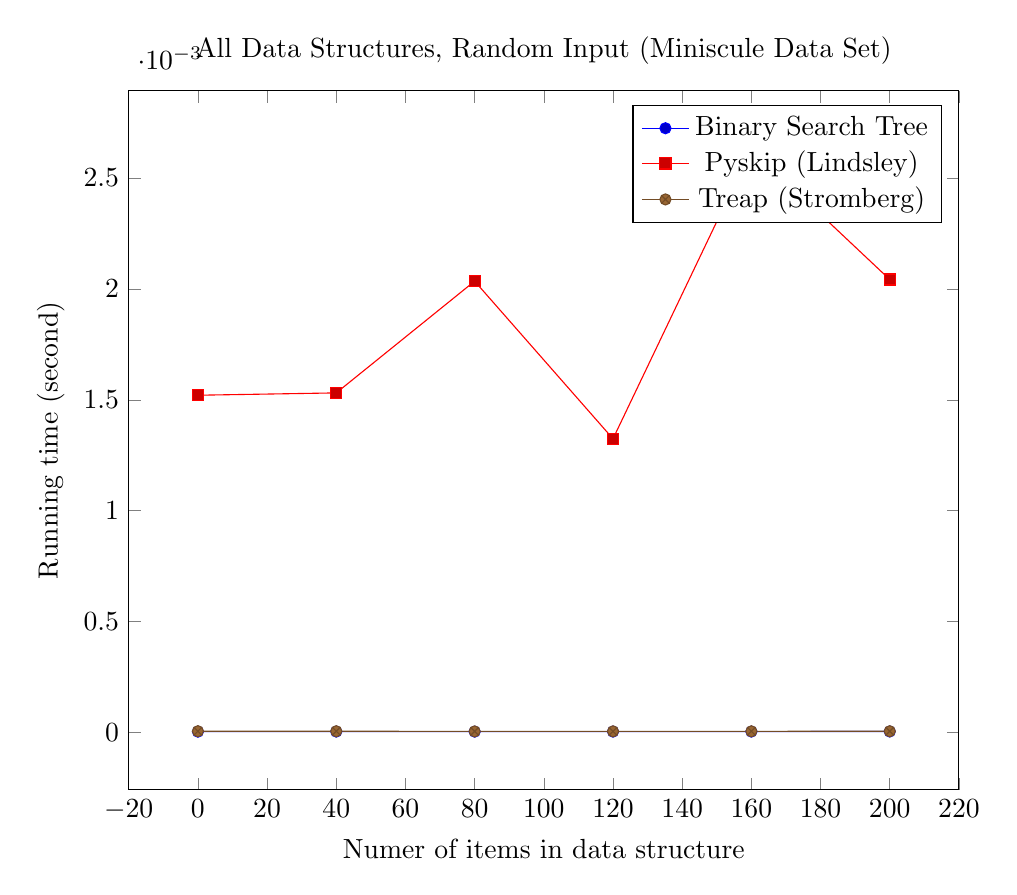
\begin{tikzpicture}
        \begin{axis}[
            xlabel={Numer of items in data structure},
            ylabel={Running time (second)},
            title={All Data Structures, Random Input (Miniscule Data Set)},
            width=\textwidth
        ]
		\addplot coordinates {
			(0, 3.463516372642639e-06)
			(40, 3.73457417572054e-06)
			(80, 3.5237514399932835e-06)
			(120, 3.73457417572054e-06)
			(160, 3.7948092430711845e-06)
			(200, 4.126102113496955e-06)
		};
		\addplot coordinates {
			(0, 0.0015205740401918494)
			(40, 0.0015310850594444814)
			(80, 0.0020349513978300316)
			(120, 0.0013241474855624103)
			(160, 0.0026300738632513364)
			(200, 0.0020423904286477946)
		};
		\addplot coordinates {
			(0, 5.481391128880908e-06)
			(40, 5.391038527846615e-06)
			(80, 4.668217719649981e-06)
			(120, 4.8489229216963635e-06)
			(160, 4.969393056408755e-06)
			(200, 5.330803460501521e-06)
		};
        \legend{Binary Search Tree, Pyskip (Lindsley), Treap (Stromberg)}
        \end{axis}
    \end{tikzpicture}
    \caption{Average of 10 operations, benchmarked every 40, starting at 0.}
\end{figure}